\chapter{Softwarová analýza}

Bude zapotřebí hlavní program (nepoptřebujující GUI), který bude zpracovávat data získaná ze senzorů a ty pak kontrolovat, zda jsou spravné. Poté přes konfigurační soubor bude periodicky načítat chtěnou hodnotu, kterou porovná s daty ze senzoru a nastaví je na světlech. Mezitím bude periodicky posílat přes UDP protokol data pro vizualizaci (vlastní komunikační protokol, který bude obsahovat, hodnoty konfiguračního souboru, poslední data ze senzorů, boolean podezdření poruchy senzoru a port pro příjem dat k ovládaní přes vizualizaci).

K aplikaci budou mít přístup dva typy lidí -- administrátor a uživatel. Na nejnižší úrovni je uživatel, který může pouze sledovat stavy světel a senzorů. Správce (technik) navíc může vypínat a zapínat celkové osvětlení, upravovat config soubor a manuálně nastavovat intenzitu osvětlení (viz \autoref{Obr-Use_Case_Diagram}). 


Seznam funkcí, které aplikace umí:

\begin{itemize}
    \item sběr procentuálních hodnot osvětlení
    \item sběr viditelnosti ze senzorů
    \item sběr požadovaných procentuálních hodnot skrz vizualizaci
    \item posílaní a následné nastavení chtěné intenzity světla
    \item kontrola senzorů - vždy po sběru dat senzorů
    \item posílaní aktualního stavu vizualizaci
    \item výpočet chtěné intenzity: vezme chtěnou základní hodnotu s configu a upraví ji podle dat získaných senzory 
    \item nastavení config souboru pomocí vizualizace
    \item ukladání dat
    \item kontrola přihlášení od vizualizace.
    \item přepočítaní intenzity (zavolané vizualizací čí změnou config souboru)
\end{itemize}

\section{Komunikace}

Komunikace s osvětlením buď pomocí bezdrátového připojení opět pomocí UDP pravděpodobně.
Jinak připojení ke světlem drátovým vedením.
Komunikace s vizualizací přes UDP

\begin{figure}[H]
    \centering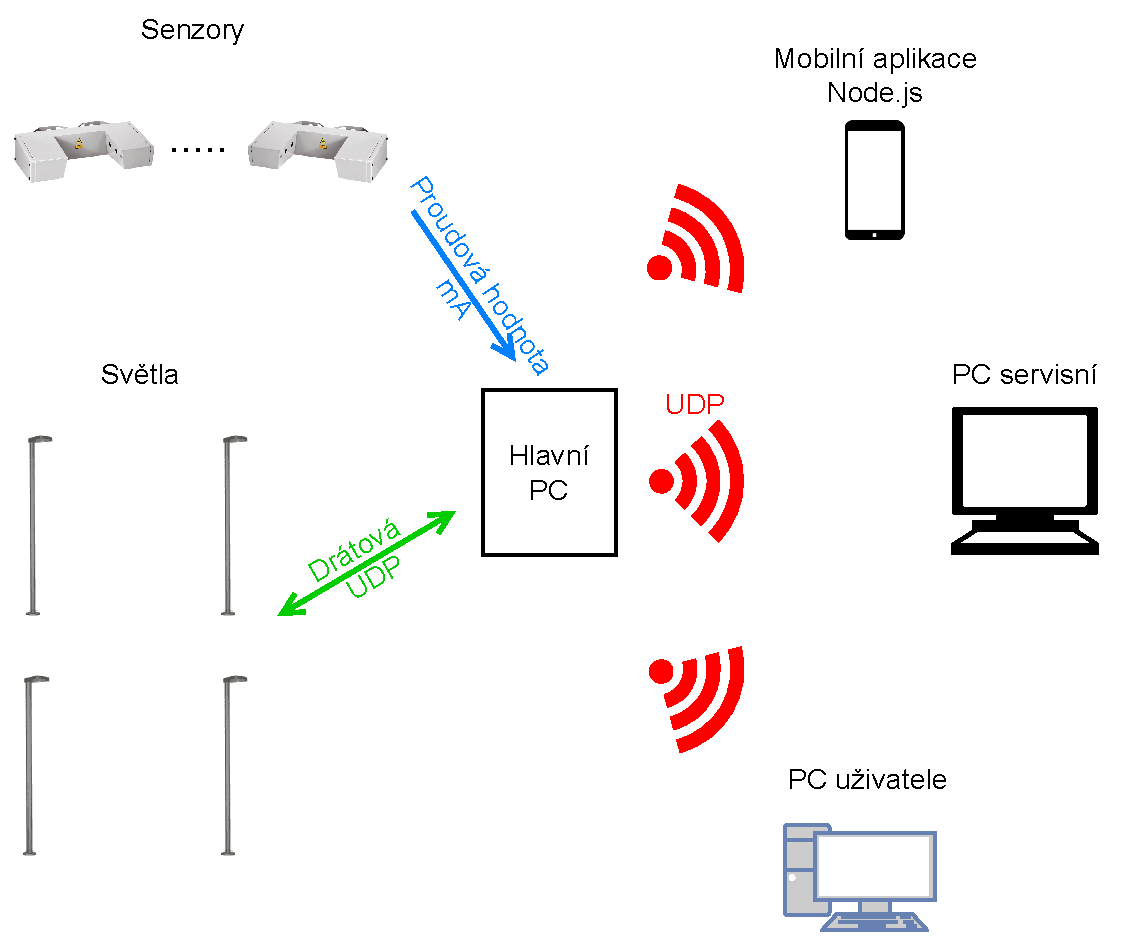
\includegraphics[width=.8\textwidth]{Figures/udp.drawio.pdf}   
    \caption{Komunikace}
    \label{Obr-Komunikace}
\end{figure}

\autoref{Obr-Komunikace} nám popisuje komunikaci našeho řešení pro osvětlení parkoviště. Senzory posílají na hlavní PC analogovou proudovou hodnotu. Pomocí drátového UDP protokolu posílají světla aktuální hodnoty na hlavní PC, který zpětně je schopný přes UDP světla ovládat a nastavovat tedy jejich hodnotu svítivosti. Dále je schopen komunikovat s PC uživatele, který má naší aplikaci vytvořenou v prostředí Promotic, případně se servisním PC, a to bezdrátově (wifi). Dále existuje možnost pomocí Node.js komunikace s mobilním telefonem, kterou momentálně nevyužíváme.



\section{Analýza dokumentů}

\section{Analýza obsahu a struktury informací}

\section{Analýza toku informací}

\section{Analýza slabých míst}


\endinput
